

\newcommand{\FeLeft}{0.60\linewidth}
\newcommand{\FeRight}{0.38\linewidth}
\newcommand{\FeCluster}{0.65\linewidth}
\newcommand{\FePlot}{0.78\linewidth}

\begin{frame}
  \frametitle<1>{Iron metal: 1$^{\mathrm{st}}$ path, 1 shell }
  \frametitle<2>{Iron metal: 2$^{\mathrm{nd}}$ path, 2 shells }
  \frametitle<3>{Iron metal: 3$^{\mathrm{rd}}$ path, 1 shell }
  \frametitle<4>{Iron metal: 4$^{\mathrm{th}}$ path, 2 shells }
  \frametitle<5>{Iron metal: 5$^{\mathrm{th}}$ path, 3 shells }
  \frametitle<6>{Iron metal: 8$^{\mathrm{th}}$ path, 4 shells }

  \begin{columns}[T]
    \begin{column}{0.60\linewidth}
      \centering\includegraphics<1>[width=\FeCluster]{images/path1_diagram}
      \centering\includegraphics<2>[width=\FeCluster]{images/path2_diagram}
      \centering\includegraphics<3>[width=\FeCluster]{images/path3_diagram}
      \centering\includegraphics<4>[width=\FeCluster]{images/path4_diagram}
      \centering\includegraphics<5>[width=\FeCluster]{images/path5_diagram}
      \centering\includegraphics<6>[width=\FeCluster]{images/path8_diagram}
      \begin{enumerate}
      \item %
        \only<1>{The first path is much, but not all, of the first peak in {\chir}.}
        \only<2>{The second path overlaps the first in {\chir}.}
        \only<3>{This path contributes little to {\chir}.}
        \only<4>{This path contributes little to {\chir}.}
        \only<5>{This 3$^{\mathrm{rd}}$ shell SS path contributes most
          of the spectral weight to the second peak of {\chir}.}
        \only<6>{The 4$^{\mathrm{th}}$ shell SS path contributes to
          the third peak in {\chir}.}\\
        {\color{Firebrick3}Degeneracy = \only<1>{8}\only<2>{6}\only<3>{24}\only<4>{48}\only<5>{12}\only<6>{24}}
      \item %
        \only<1>{The first shell XANES calculation shows little of the
          structure.}
        \only<2>{The XANES calculation begins to show the structure of
          the spectrum.}
        \only<3>{The contribution from this path and all higher order
          paths scattering among these atoms is in the first shell
          XANES calculation.}
        \only<4>{The contribution from this path and all higher order
          paths scattering among these the first two shells is in the
          second shell XANES calculation.}
        \only<5>{The first peak after the edge in the XANES is
          sharpened considerably by the addition of this shell.}
        \only<6>{Including this shell in the XANES calculation broadens
          the peak above the edge somewhat.  It also introduces the
          second shoulder.}
      \end{enumerate}
    \end{column}
    \begin{column}{0.38\linewidth}
      \centering
      \includegraphics<1>[width=\FePlot]{images/path1}
      \includegraphics<2>[width=\FePlot]{images/path2}
      \includegraphics<3>[width=\FePlot]{images/path3}
      \includegraphics<4>[width=\FePlot]{images/path4}
      \includegraphics<5>[width=\FePlot]{images/path5}
      \includegraphics<6>[width=\FePlot]{images/path8}

      \centering\color{Green4}\texttt{`feff000{\only<1>{1}\only<2>{2}\only<3>{3}\only<4>{4}\only<5>{5}\only<6>{8}}.dat'}
      %\only<2>{\color{Green4}\texttt{`feff0002.dat'}}
      %\only<3>{\color{Green4}\texttt{`feff0003.dat'}}
      %\only<4>{\color{Green4}\texttt{`feff0004.dat'}}
      %\only<5>{\color{Green4}\texttt{`feff0005.dat'}}
      %\only<6>{\color{Green4}\texttt{`feff0008.dat'}}

      \bigskip

      \includegraphics<1>[width=\FePlot]{images/xanes_shell1}
      \includegraphics<2>[width=\FePlot]{images/xanes_shell2}
      \includegraphics<3>[width=\FePlot]{images/xanes_shell1}
      \includegraphics<4>[width=\FePlot]{images/xanes_shell2}
      \includegraphics<5>[width=\FePlot]{images/xanes_shell3}
      \includegraphics<6>[width=\FePlot]{images/xanes_shell4}

      \centering{\color{blue}XANES}

      \bigskip

      ~

      \bigskip

      ~

    \end{column}
  \end{columns}
\end{frame}



\begin{frame}
  \frametitle{Iron metal: 10$^{\mathrm{th}}$ path + MS, 5 shells}
  \begin{columns}[T]
    \begin{column}{0.38\linewidth}
      \begin{center}
        5$^{\mathrm{th}}$ shell EXAFS

        \medskip

        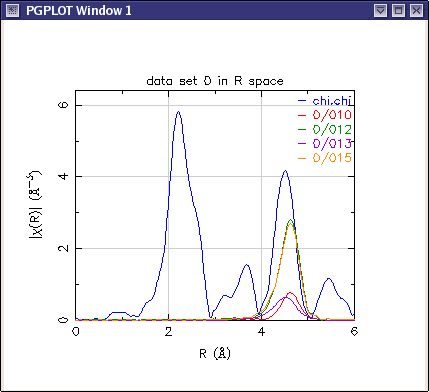
\includegraphics[width=0.8\linewidth]{images/path10}

        Magnitude

        \bigskip

        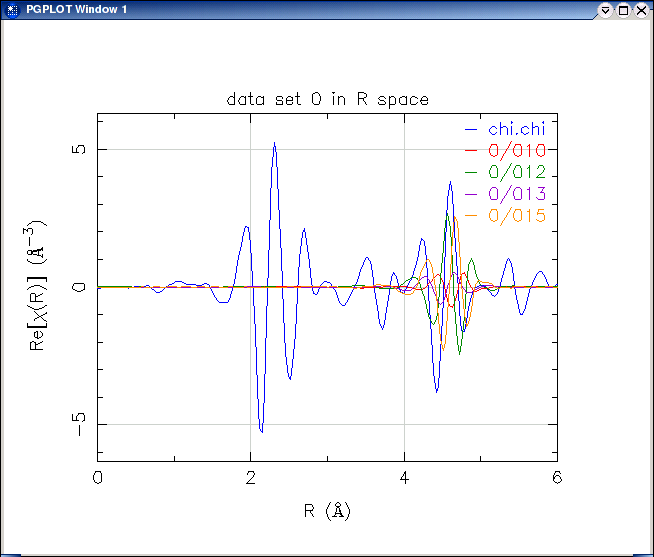
\includegraphics[width=0.8\linewidth]{images/path10_re}

        Real part
      \end{center}
    \end{column}
    \begin{column}{0.62\linewidth}
      There are several MS geometries with the same path length as the
      5$^{\mathrm{th}}$ shell SS path.  Some are \emph{bigger} than
      the SS path!

      \bigskip

      \begin{block}{Convergence}
        \centering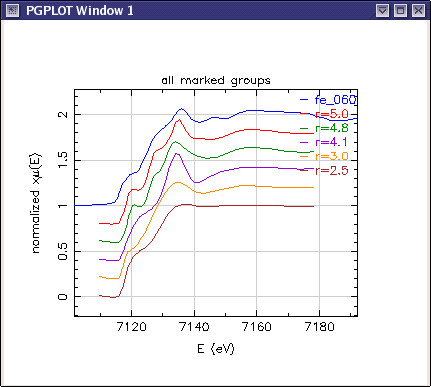
\includegraphics[width=0.7\linewidth]{images/xanes_convergence}
      \end{block}
    \end{column}
  \end{columns}
\end{frame}


%%% Local Variables:
%%% mode: latex
%%% TeX-master: t
%%% End:
